% Options for packages loaded elsewhere
\PassOptionsToPackage{unicode}{hyperref}
\PassOptionsToPackage{hyphens}{url}
%
\documentclass[
]{article}
\usepackage{amsmath,amssymb}
\usepackage{lmodern}
\usepackage{iftex}
\ifPDFTeX
  \usepackage[T1]{fontenc}
  \usepackage[utf8]{inputenc}
  \usepackage{textcomp} % provide euro and other symbols
\else % if luatex or xetex
  \usepackage{unicode-math}
  \defaultfontfeatures{Scale=MatchLowercase}
  \defaultfontfeatures[\rmfamily]{Ligatures=TeX,Scale=1}
\fi
% Use upquote if available, for straight quotes in verbatim environments
\IfFileExists{upquote.sty}{\usepackage{upquote}}{}
\IfFileExists{microtype.sty}{% use microtype if available
  \usepackage[]{microtype}
  \UseMicrotypeSet[protrusion]{basicmath} % disable protrusion for tt fonts
}{}
\makeatletter
\@ifundefined{KOMAClassName}{% if non-KOMA class
  \IfFileExists{parskip.sty}{%
    \usepackage{parskip}
  }{% else
    \setlength{\parindent}{0pt}
    \setlength{\parskip}{6pt plus 2pt minus 1pt}}
}{% if KOMA class
  \KOMAoptions{parskip=half}}
\makeatother
\usepackage{xcolor}
\IfFileExists{xurl.sty}{\usepackage{xurl}}{} % add URL line breaks if available
\IfFileExists{bookmark.sty}{\usepackage{bookmark}}{\usepackage{hyperref}}
\hypersetup{
  pdftitle={Title Goes Here},
  pdfkeywords={keyword 1; keyword 2; keyword 3},
  hidelinks,
  pdfcreator={LaTeX via pandoc}}
\urlstyle{same} % disable monospaced font for URLs
\usepackage[margin=1in]{geometry}
\usepackage{longtable,booktabs,array}
\usepackage{calc} % for calculating minipage widths
% Correct order of tables after \paragraph or \subparagraph
\usepackage{etoolbox}
\makeatletter
\patchcmd\longtable{\par}{\if@noskipsec\mbox{}\fi\par}{}{}
\makeatother
% Allow footnotes in longtable head/foot
\IfFileExists{footnotehyper.sty}{\usepackage{footnotehyper}}{\usepackage{footnote}}
\makesavenoteenv{longtable}
\usepackage{graphicx}
\makeatletter
\def\maxwidth{\ifdim\Gin@nat@width>\linewidth\linewidth\else\Gin@nat@width\fi}
\def\maxheight{\ifdim\Gin@nat@height>\textheight\textheight\else\Gin@nat@height\fi}
\makeatother
% Scale images if necessary, so that they will not overflow the page
% margins by default, and it is still possible to overwrite the defaults
% using explicit options in \includegraphics[width, height, ...]{}
\setkeys{Gin}{width=\maxwidth,height=\maxheight,keepaspectratio}
% Set default figure placement to htbp
\makeatletter
\def\fps@figure{htbp}
\makeatother
\setlength{\emergencystretch}{3em} % prevent overfull lines
\providecommand{\tightlist}{%
  \setlength{\itemsep}{0pt}\setlength{\parskip}{0pt}}
\setcounter{secnumdepth}{5}
\newlength{\cslhangindent}
\setlength{\cslhangindent}{1.5em}
\newlength{\csllabelwidth}
\setlength{\csllabelwidth}{3em}
\newlength{\cslentryspacingunit} % times entry-spacing
\setlength{\cslentryspacingunit}{\parskip}
\newenvironment{CSLReferences}[2] % #1 hanging-ident, #2 entry spacing
 {% don't indent paragraphs
  \setlength{\parindent}{0pt}
  % turn on hanging indent if param 1 is 1
  \ifodd #1
  \let\oldpar\par
  \def\par{\hangindent=\cslhangindent\oldpar}
  \fi
  % set entry spacing
  \setlength{\parskip}{#2\cslentryspacingunit}
 }%
 {}
\usepackage{calc}
\newcommand{\CSLBlock}[1]{#1\hfill\break}
\newcommand{\CSLLeftMargin}[1]{\parbox[t]{\csllabelwidth}{#1}}
\newcommand{\CSLRightInline}[1]{\parbox[t]{\linewidth - \csllabelwidth}{#1}\break}
\newcommand{\CSLIndent}[1]{\hspace{\cslhangindent}#1}
\ifLuaTeX
  \usepackage{selnolig}  % disable illegal ligatures
\fi

\title{Title Goes Here}
\author{true \and true}
\date{09 June, 2022}

\begin{document}
\maketitle
\begin{abstract}
Text of abstract
\end{abstract}

{
\setcounter{tocdepth}{2}
\tableofcontents
}
Keywords: keyword 1; keyword 2; keyword 3

Highlights: These are the highlights.

\hypertarget{introduction}{%
\section{Introduction}\label{introduction}}

Here is a citation (Marwick, 2017)

\hypertarget{background}{%
\section{Background}\label{background}}

\hypertarget{methods}{%
\section{Methods}\label{methods}}

\hypertarget{results}{%
\section{Results}\label{results}}

\begin{table}

\caption{\label{tab:type}Type of tools}
\centering
\begin{tabular}[t]{l|r}
\hline
typedb & Freq\\
\hline
Débris & 2\\
\hline
Denticulé & 9\\
\hline
Eclat & 50\\
\hline
Eclat  de ravivage & 1\\
\hline
Eclat laminaire & 3\\
\hline
Encoche & 10\\
\hline
Fragment & 13\\
\hline
Grand fragment & 4\\
\hline
Grand Fragment & 1\\
\hline
Grattoir & 2\\
\hline
Lame & 22\\
\hline
Lamelle & 10\\
\hline
Nucléus & 5\\
\hline
Perçoir & 1\\
\hline
Pointe & 1\\
\hline
Racloir & 7\\
\hline
\end{tabular}
\end{table}

A lot of technological types do not have a platform present (\ref{fig:hist1}). However, when we look at the types which have platforms, we see that most of them are plain.

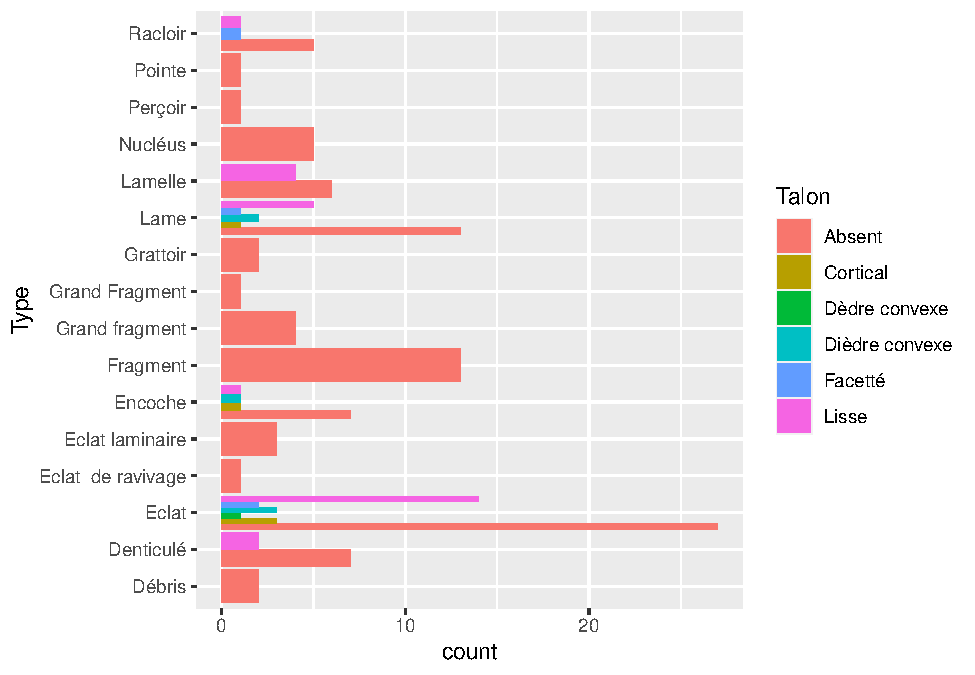
\includegraphics{../figures/hist1-1.pdf}

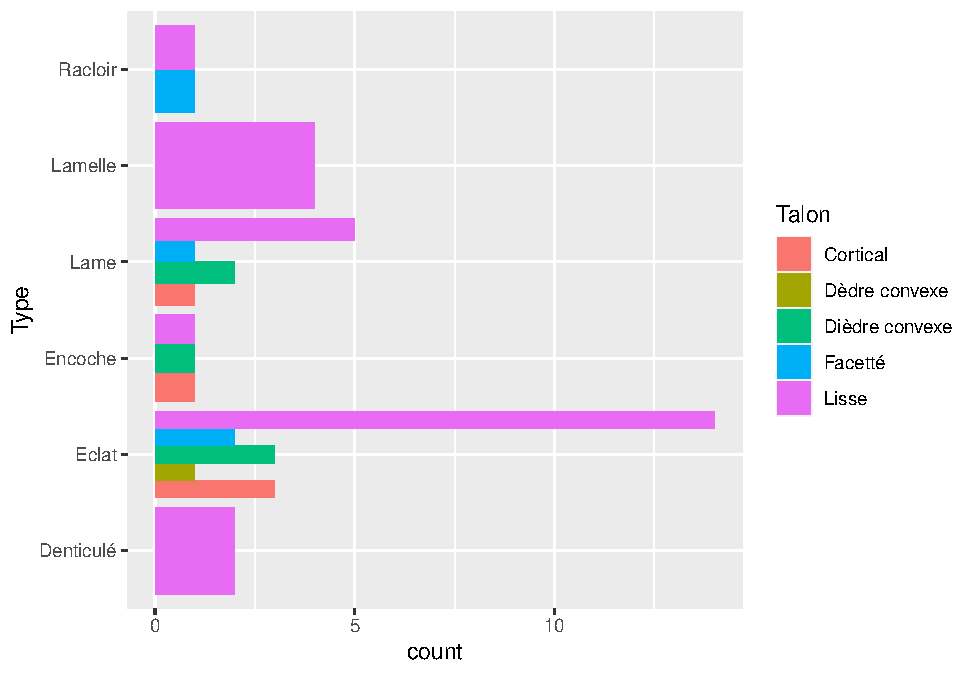
\includegraphics{../figures/hist2-1.pdf}

\hypertarget{discussion}{%
\section{Discussion}\label{discussion}}

\hypertarget{conclusion}{%
\section{Conclusion}\label{conclusion}}

\hypertarget{acknowledgements}{%
\section{Acknowledgements}\label{acknowledgements}}

\newpage

\hypertarget{references}{%
\section{References}\label{references}}

\hypertarget{refs}{}
\begin{CSLReferences}{1}{0}
\leavevmode\vadjust pre{\hypertarget{ref-Marwick2017}{}}%
Marwick, B., 2017. Computational reproducibility in archaeological research: Basic principles and a case study of their implementation. Journal of Archaeological Method and Theory 24, 424--450. \url{https://doi.org/10.1007/s10816-015-9272-9}

\end{CSLReferences}

\newpage

\hypertarget{colophon}{%
\subsubsection{Colophon}\label{colophon}}

This report was generated on 2022-06-09 14:20:20 using the following computational environment and dependencies:

\begin{verbatim}
#> - Session info ---------------------------------------------------------------
#>  setting  value
#>  version  R version 4.1.3 (2022-03-10)
#>  os       Windows 10 x64 (build 19043)
#>  system   x86_64, mingw32
#>  ui       RTerm
#>  language (EN)
#>  collate  English_United States.1252
#>  ctype    English_United States.1252
#>  tz       Europe/London
#>  date     2022-06-09
#>  pandoc   2.17.1.1 @ C:/Program Files/RStudio/bin/quarto/bin/ (via rmarkdown)
#> 
#> - Packages -------------------------------------------------------------------
#>  package     * version date (UTC) lib source
#>  assertthat    0.2.1   2019-03-21 [1] CRAN (R 4.1.3)
#>  backports     1.4.1   2021-12-13 [1] CRAN (R 4.1.2)
#>  bit           4.0.4   2020-08-04 [1] CRAN (R 4.1.3)
#>  bit64         4.0.5   2020-08-30 [1] CRAN (R 4.1.3)
#>  bookdown      0.26    2022-04-15 [1] CRAN (R 4.1.3)
#>  brio          1.1.3   2021-11-30 [1] CRAN (R 4.1.3)
#>  broom         0.8.0   2022-04-13 [1] CRAN (R 4.1.3)
#>  cachem        1.0.6   2021-08-19 [1] CRAN (R 4.1.3)
#>  callr         3.7.0   2021-04-20 [1] CRAN (R 4.1.3)
#>  cellranger    1.1.0   2016-07-27 [1] CRAN (R 4.1.3)
#>  cli           3.2.0   2022-02-14 [1] CRAN (R 4.1.3)
#>  colorspace    2.0-3   2022-02-21 [1] CRAN (R 4.1.3)
#>  crayon        1.5.1   2022-03-26 [1] CRAN (R 4.1.3)
#>  DBI           1.1.2   2021-12-20 [1] CRAN (R 4.1.3)
#>  dbplyr        2.1.1   2021-04-06 [1] CRAN (R 4.1.3)
#>  desc          1.4.1   2022-03-06 [1] CRAN (R 4.1.3)
#>  devtools      2.4.3   2021-11-30 [1] CRAN (R 4.1.3)
#>  digest        0.6.29  2021-12-01 [1] CRAN (R 4.1.3)
#>  dplyr       * 1.0.9   2022-04-28 [1] CRAN (R 4.1.3)
#>  ellipsis      0.3.2   2021-04-29 [1] CRAN (R 4.1.3)
#>  evaluate      0.15    2022-02-18 [1] CRAN (R 4.1.3)
#>  fansi         1.0.3   2022-03-24 [1] CRAN (R 4.1.3)
#>  farver        2.1.0   2021-02-28 [1] CRAN (R 4.1.3)
#>  fastmap       1.1.0   2021-01-25 [1] CRAN (R 4.1.3)
#>  forcats     * 0.5.1   2021-01-27 [1] CRAN (R 4.1.3)
#>  fs            1.5.2   2021-12-08 [1] CRAN (R 4.1.3)
#>  generics      0.1.2   2022-01-31 [1] CRAN (R 4.1.3)
#>  ggplot2     * 3.3.6   2022-05-03 [1] CRAN (R 4.1.3)
#>  glue          1.6.2   2022-02-24 [1] CRAN (R 4.1.3)
#>  gtable        0.3.0   2019-03-25 [1] CRAN (R 4.1.3)
#>  haven         2.5.0   2022-04-15 [1] CRAN (R 4.1.3)
#>  here          1.0.1   2020-12-13 [1] CRAN (R 4.1.3)
#>  highr         0.9     2021-04-16 [1] CRAN (R 4.1.3)
#>  hms           1.1.1   2021-09-26 [1] CRAN (R 4.1.3)
#>  htmltools     0.5.2   2021-08-25 [1] CRAN (R 4.1.3)
#>  httr          1.4.3   2022-05-04 [1] CRAN (R 4.1.3)
#>  jsonlite      1.8.0   2022-02-22 [1] CRAN (R 4.1.3)
#>  knitr       * 1.39    2022-04-26 [1] CRAN (R 4.1.3)
#>  labeling      0.4.2   2020-10-20 [1] CRAN (R 4.1.1)
#>  lifecycle     1.0.1   2021-09-24 [1] CRAN (R 4.1.3)
#>  lubridate     1.8.0   2021-10-07 [1] CRAN (R 4.1.3)
#>  magrittr      2.0.3   2022-03-30 [1] CRAN (R 4.1.3)
#>  memoise       2.0.1   2021-11-26 [1] CRAN (R 4.1.3)
#>  modelr        0.1.8   2020-05-19 [1] CRAN (R 4.1.3)
#>  munsell       0.5.0   2018-06-12 [1] CRAN (R 4.1.3)
#>  pillar        1.7.0   2022-02-01 [1] CRAN (R 4.1.3)
#>  pkgbuild      1.3.1   2021-12-20 [1] CRAN (R 4.1.3)
#>  pkgconfig     2.0.3   2019-09-22 [1] CRAN (R 4.1.3)
#>  pkgload       1.2.4   2021-11-30 [1] CRAN (R 4.1.3)
#>  prettyunits   1.1.1   2020-01-24 [1] CRAN (R 4.1.3)
#>  processx      3.5.3   2022-03-25 [1] CRAN (R 4.1.3)
#>  ps            1.7.0   2022-04-23 [1] CRAN (R 4.1.3)
#>  purrr       * 0.3.4   2020-04-17 [1] CRAN (R 4.1.3)
#>  R6            2.5.1   2021-08-19 [1] CRAN (R 4.1.3)
#>  readr       * 2.1.2   2022-01-30 [1] CRAN (R 4.1.3)
#>  readxl        1.4.0   2022-03-28 [1] CRAN (R 4.1.3)
#>  remotes       2.4.2   2021-11-30 [1] CRAN (R 4.1.3)
#>  reprex        2.0.1   2021-08-05 [1] CRAN (R 4.1.3)
#>  rlang         1.0.2   2022-03-04 [1] CRAN (R 4.1.3)
#>  rmarkdown     2.14    2022-04-25 [1] CRAN (R 4.1.3)
#>  rprojroot     2.0.3   2022-04-02 [1] CRAN (R 4.1.3)
#>  rstudioapi    0.13    2020-11-12 [1] CRAN (R 4.1.3)
#>  rvest         1.0.2   2021-10-16 [1] CRAN (R 4.1.3)
#>  scales        1.2.0   2022-04-13 [1] CRAN (R 4.1.3)
#>  sessioninfo   1.2.2   2021-12-06 [1] CRAN (R 4.1.3)
#>  stringi       1.7.6   2021-11-29 [1] CRAN (R 4.1.2)
#>  stringr     * 1.4.0   2019-02-10 [1] CRAN (R 4.1.3)
#>  testthat      3.1.4   2022-04-26 [1] CRAN (R 4.1.3)
#>  tibble      * 3.1.7   2022-05-03 [1] CRAN (R 4.1.3)
#>  tidyr       * 1.2.0   2022-02-01 [1] CRAN (R 4.1.3)
#>  tidyselect    1.1.2   2022-02-21 [1] CRAN (R 4.1.3)
#>  tidyverse   * 1.3.1   2021-04-15 [1] CRAN (R 4.1.3)
#>  tzdb          0.3.0   2022-03-28 [1] CRAN (R 4.1.3)
#>  usethis       2.1.5   2021-12-09 [1] CRAN (R 4.1.3)
#>  utf8          1.2.2   2021-07-24 [1] CRAN (R 4.1.3)
#>  vctrs         0.4.1   2022-04-13 [1] CRAN (R 4.1.3)
#>  vroom         1.5.7   2021-11-30 [1] CRAN (R 4.1.3)
#>  withr         2.5.0   2022-03-03 [1] CRAN (R 4.1.3)
#>  xfun          0.31    2022-05-10 [1] CRAN (R 4.1.3)
#>  xml2          1.3.3   2021-11-30 [1] CRAN (R 4.1.3)
#>  yaml          2.3.5   2022-02-21 [1] CRAN (R 4.1.2)
#> 
#>  [1] C:/Users/Youssef/OneDrive/Documents/R/win-library/4.1
#>  [2] C:/Program Files/R/R-4.1.3/library
#> 
#> ------------------------------------------------------------------------------
\end{verbatim}

The current Git commit details are:

\begin{verbatim}
#> Local:    main C:/Users/Youssef/OneDrive/Bureau/ClassRstudio/ClassRstudio
#> Remote:   main @ origin (https://github.com/YDjellal1/ClassRstudio.git)
#> Head:     [2adb17a] 2022-05-19: second
\end{verbatim}

\end{document}
